% ! Tex program = xelatex
\documentclass[a4paper,landscape]{article}
\PassOptionsToPackage{quiet}{fontspec}
\usepackage[UTF8]{ctex}
%! Tex program = xelatex
% \documentclass{article}
%中文
%\usepackage[UTF8]{ctex}
%数学公式
\usepackage{amsmath,amssymb}
%\usepackage{ntheorem}
% \usepackage[framemethod=TikZ]{mdframed}
\usepackage{amsthm}
%边界
\usepackage[letterpaper,top=3cm,bottom=3cm,left=2cm,right=2cm,marginparwidth=1.75cm]{geometry}%table package
%Table
\usepackage{multirow,booktabs}
\usepackage{makecell}
%字体颜色
\usepackage{color}
\usepackage[dvipsnames]{xcolor}  % 更全的色系
%代码
\usepackage[OT1]{fontenc}
% MATLAB 代码风格
% \usepackage[framed,numbered,autolinebreaks,useliterate]{/Users/anye_zhenhaoyu/Desktop/Latex/mcode}
\usepackage{listings}
\usepackage{algorithm}
\usepackage{algorithmic}
\usepackage{pythonhighlight} % Python
%插图
\usepackage{graphicx}
%改变item格式
\usepackage{enumerate}
%物理
\usepackage{physics}
%extra arrows
\usepackage{extarrows}
% caption(居中指令)
\usepackage[justification=centering]{caption}
% \usepackage{caption}
% htpb
\usepackage{stfloats}
% pdf 拼接
\usepackage{pdfpages}
% 超链接url
\usepackage{url}
% \usepackage{tikz}
\usepackage{pgfplots}
\pgfplotsset{compat=newest}
\usepackage[colorlinks=true, allcolors=blue]{hyperref}
\usepackage{setspace}

% --------------definations-------------- %
\def\*#1{\boldsymbol{#1}}
\def\+#1{\mathcal{#1}} 
\def\-#1{\bar{#1}}
% Domains
\def\RR{\mathbb{R}}
\def\CC{\mathbb{C}}
\def\NN{\mathbb{N}}
\def\ZZ{\mathbb{Z}}
% Newcommand
\newcommand{\inner}[2]{\langle #1,#2\rangle} 
\newcommand{\numP}{\#\mathbf{P}} 
\renewcommand{\P}{\mathbf{P}}
\newcommand{\Var}[2][]{\mathbf{Var}_{#1}\left[#2\right]}
\newcommand{\E}[2][]{\mathbf{E}_{#1}\left[#2\right]}
\renewcommand{\emptyset}{\varnothing}
\newcommand{\ol}{\overline}
\newcommand{\argmin}{\mathop{\arg\min}}
\newcommand{\argmax}{\mathop{\arg\max}}
\renewcommand{\abs}[1]{\qty|#1|}
\newcommand{\defeq}{\triangleq} % triangle over =
\def\deq{\xlongequal{def}} % 'def' over =
\def\LHS{\text{LHS}}
\def\RHS{\text{RHS}}
\def\angbr#1{\langle#1\rangle} % <x>

\def\Esolve{\textcolor{blue}{Solve: }}
\def\Eproof{\textcolor{blue}{Proof: }}
\def\case#1{\textcolor{blue}{Case \uppercase\expandafter{\romannumeral#1}: }}

\newtheorem{lemma}{Lemma}
\newtheorem{thm}{Theorem}
\newtheorem{defi}{Definition}
\newtheorem{prp}{Proposition}
\newenvironment{md}{\begin{mdframed}}{\end{mdframed}}

\date{\today}
\usepackage{fancyhdr}
\pagestyle{fancy}
\fancyhead[L]{\slshape{Haoyu Zhen}}
\fancyhead[R]{{\today}}

% \begin{document}
% \title{<++>}
\author{Haoyu Zhen}
% \maketitle
\setlength{\parindent}{0pt}
\setstretch{1.2}
% \end{document}



\usepackage{titlesec}
% \titleformat*{\section}{\scriptsize\bfseries}
% \titleformat*{\subsection}{\scriptsize\bfseries}
% \titleformat*{\subsubsection}{\scriptsize\bfseries}
% \titlespacing{\section}{0.5pt}{\parskip}{-\parskip}
% \titlespacing{\subsection}{0.5pt}{\parskip}{-\parskip}
\graphicspath{{figs/}}

\usepackage{cellspace}%
% \setlength\cellspacetoplimit{2pt}
% \setlength\cellspacebottomlimit{6pt}
\usepackage{makecell}
\usepackage{enumitem}

% \setcellgapes{3pt}

\begin{document}
\setlength{\abovedisplayskip}{0.5pt}
\setlength{\belowdisplayskip}{0.5pt}

\newcommand{\ds}{\displaystyle}
\title{\vspace{0.4cm} AI2611 CheatSheet}
\maketitle
\section*{\centering Preface}
\begin{minipage}[t]{0.49\linewidth}
	\subsection*{\centering \vspace{0.3cm} Introduction}
	\setlist{nosep,leftmargin=20pt}
	\begin{itemize}
		\item
		      My Machine Learning Lecture Notes (更丰富的版本,适合学习这门课):\\
		      \href{https://github.com/anyeZHY/Self-Learning/blob/main/CS229/MyNotes/ML.pdf}{Self-Learning/CS229/MyNotes/ML.pdf}
		\item
		      \LaTeX\, code of the CheatSheet is available at:\\
		      \href{https://github.com/anyeZHY/SJTU-Course-Stack}{SJTU-Course-Stack/AI2611/CheatSheet}
		\item
		      CheatSheet为2022版(非常少较草率,当然有部分超纲,不适合用于学习)。
	\end{itemize}
\end{minipage}
\begin{minipage}[t]{0.49\linewidth}
	\subsection*{\centering \vspace{0.3cm} Ackonwledgement}
	\setlist{nosep,leftmargin=20pt}
	\begin{itemize}
		\item CS229, Stanford University. (Foundation, Kernel Method, GMM)
		\item CS231n, Stanford University. (Deep Learning)
		\item CS189, UC Berkeley. (Random Forest)
		\item Understanding Machine Learning, Cambridge University. (Linear Regression, KNN, SVM, K-means, PCA)
		\item AI2611, Shanghai Jiao Tong University. (中文部分, Spectral, Dimensionality Reduction)
	\end{itemize}
\end{minipage}

\clearpage

\begin{tiny}
	\renewcommand{\section}[1]{{$\S$ \scriptsize\bfseries #1}}
	\renewcommand{\subsection}[1]{{\scriptsize\bfseries #1}}
	\setlist{nosep,leftmargin=10pt}
	\begin{multicols}{4}
		\section{Foundation}

		\begin{minipage}[]{0.58\linewidth}
			监督学习、无监督学习(聚类、降维)\\独立同分布;最小化范化误差
		\end{minipage}
		\begin{minipage}[p]{0.38\linewidth}
			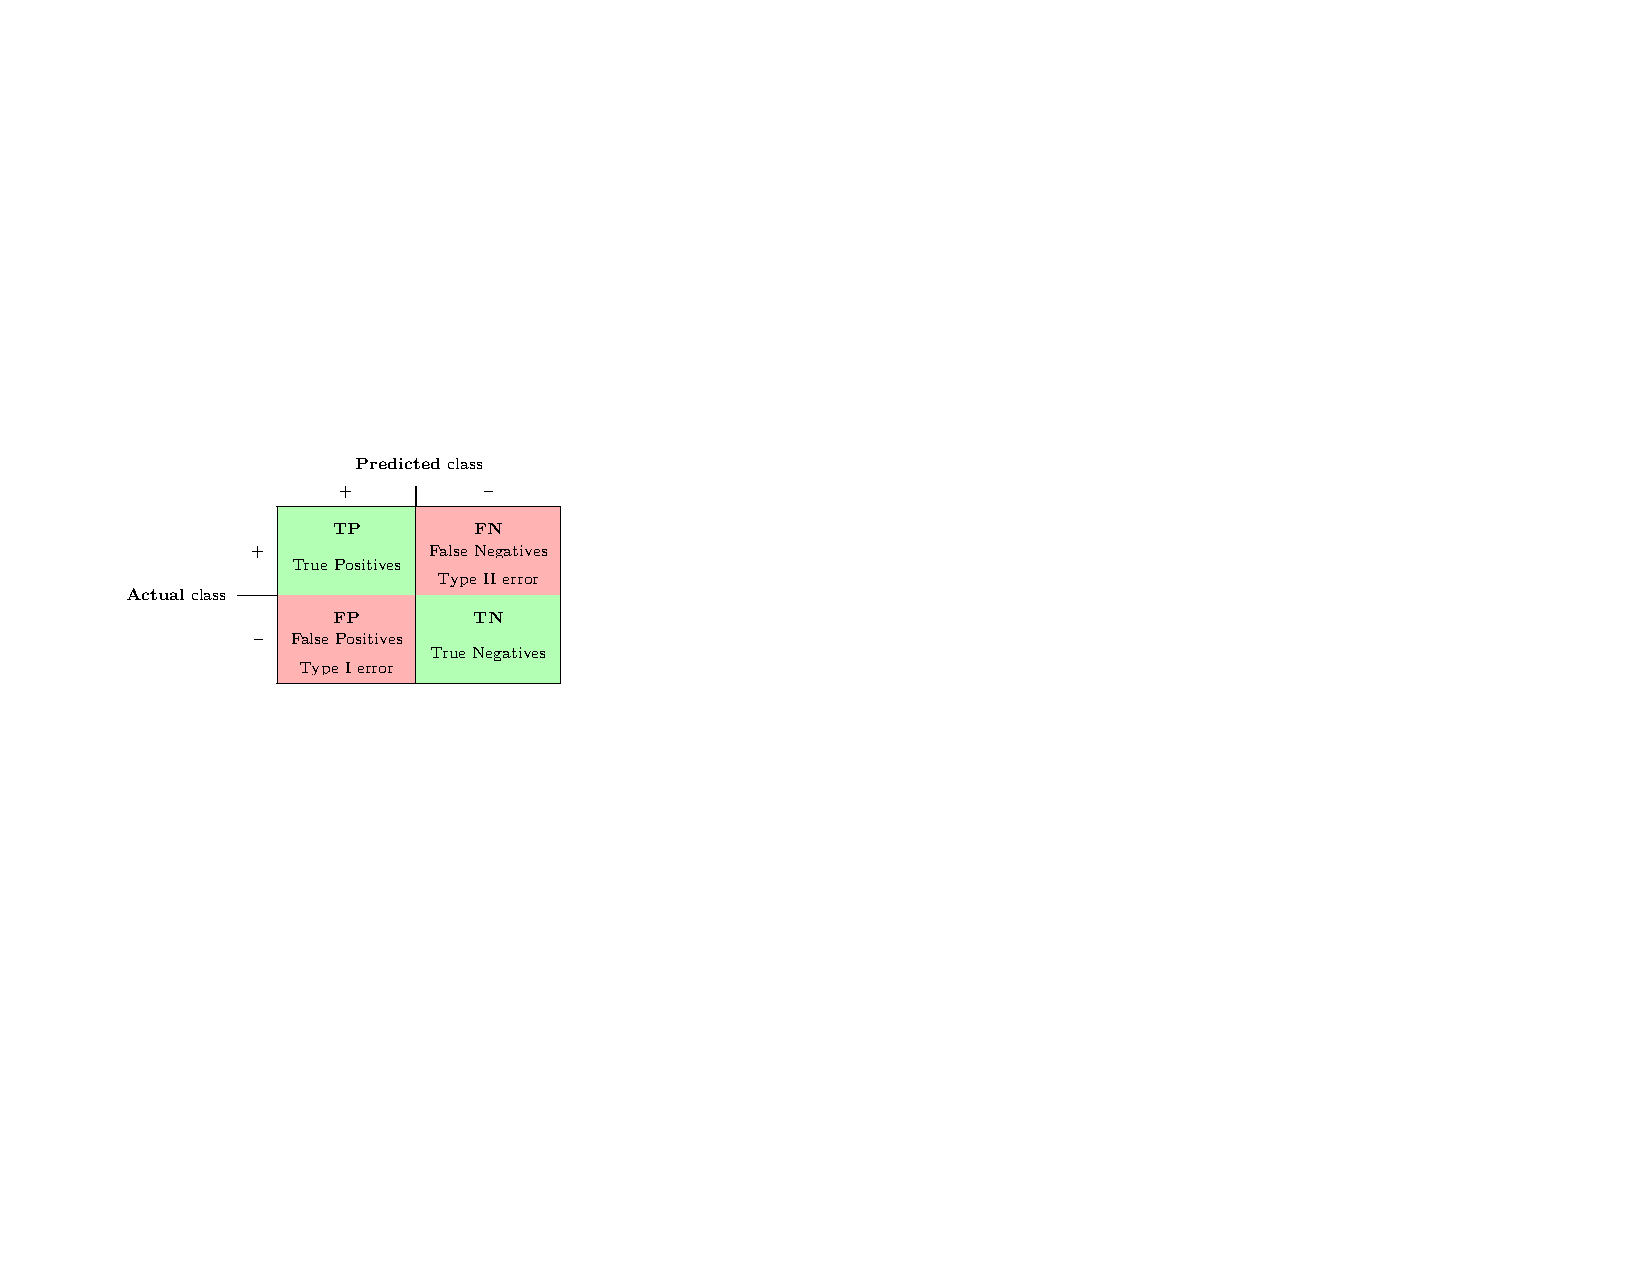
\includegraphics[width=\linewidth]{sensitivity.pdf}
		\end{minipage}

		\resizebox{\linewidth}{!}{
			\begin{tabular}{|c|c|l|} \hline
				% 			\rule{0pt}{4.5ex}
				\textbf{Metric}                                                                                   & \textbf{Formula} & \textbf{Interpretation} \\ \hline
				\rule[-4ex]{0pt}{9ex}
				准确率 (Accuracy)                                                                                    &
				$\cfrac{\mathrm{TP}+\mathrm{TN}}{\mathrm{TP}+\mathrm{TN}+\mathrm{FP}+\mathrm{FN}}$                &
				Overall performance of model                                                                                                                   \\ \hline
				\rule[-4ex]{0pt}{9ex}
				查准率 (Precision)                                                                                   &
				$\cfrac{\mathrm{TP}}{\mathrm{TP}+\mathrm{FP}}$                                                    &
				How accurate the positive predictions are                                                                                                      \\ \hline
				\rule[-4ex]{0pt}{9ex}
				通过率、查全率 (Recall Sensitivity)                                                                      &
				$\cfrac{\mathrm{TP}}{\mathrm{TP}+\mathrm{FN}}$                                                    &
				Coverage of actual positive sample                                                                                                             \\ \hline
				\rule[-4ex]{0pt}{9ex}
				假阳率 (FPR)                                                                                         &
				$\cfrac{\mathrm{FP}}{\mathrm{TN}+\mathrm{FP}}$                                                    &
				\\ \hline
				\rule[-4ex]{0pt}{9ex}
				F1 score                                                                                          &
				$\cfrac{2\mathrm{TP}}{\text{样例总数}+\mathrm{TP}-\mathrm{TN}}$                                       &
				Hybrid metric useful for unbalanced classes                                                                                                    \\ \hline
				\rule[-4ex]{0pt}{9ex}
				$F_\beta$ score                                                                                   &
				$\cfrac{(1+\beta^2)\times\mathrm{Pre}\times\mathrm{Rec}}{\beta^2\times\mathrm{Pre}+\mathrm{Rec}}$ &
				Precision and Recall
				\\ \hline
			\end{tabular}
		}

		在不同的阈值下可以得到不同的TPR和FPR值,将它们在图中绘制出来,并依次连接起来就得到了ROC曲线,阈值取值越多,ROC曲线越平滑。AUC:ROC曲线下的面积


		\textbf{模型选择:}
		留出法(hold-out,保持数据分布的一致性,多次重复划分取平均值)、
		交叉验证法(留一法,10-fold,更接近期望评估的模型,但计算量巨大;测试集只包含一个数据,无法分层采样,测试误差率区别较大;)、
		自助法(bootstrap,有放回采样,训练集中数据存在重复,适合小规模数据集)

		\textbf{误差-方差分解}
		\[
			\begin{aligned}
				E(f;D) & =\mathrm{bias}^2+\mathrm{variance}+\mathrm{error}^2
				\\&=(\bar{f}(x)-y)^2+\mathbb{E}_D[f(x; D)-\bar{f}(x)]+\mathbb{E}_D[(y_D-y)^2]
			\end{aligned}
		\]
		\section{Linear Regression}

		Loss function: $\+L_\+S(h)=\frac{1}{m}\sum_{i=1}^m(h(\*x)-\*y)^2$.
		Solve $A\*w=\*b$ where $A\deq\sum\*x_i\*x_i^T=XX^T$ and $\*b\deq\sum y_i\*x_i=X^T\*y$.

		\begin{thm}
			$\omega=(X^TX)^{-1}X^T\*y$. 优点:single-shot算法,易于实现;缺点:伪逆计算量大没可能导致数值不稳定(奇异矩阵)。
		\end{thm}

		\begin{thm}
			\label{non-inv}
			Eigenvalue decomposition:
			$A=VD^+V^T$ where $D$ is a diagnonal matrix and  $V$ is an orthonormal matrix.
			Define $D^+$ to be the diagonal matrix: $D^+_{i,i}=0$ if  $D_{i,i}=0$ otherwise  $D^+_{i,i}=\flatfrac{1}{D_{i,i}}$.
			Then, $A\*{\hat{w}}=\*b$ where $\*{\hat{w}}=VD^+V^T\*b$.
		\end{thm}

		\begin{remark}
			\textbf{Gradient Descent}. 优点:收敛快,易于实现;缺点:批量更新,可伸缩性问题。
		\end{remark}
		概率解释:$y|x;\theta\sim\+N(0,\sigma)$. Loss function 为最大似然的结果,分类器为$E[y|x]$。

		\subsection{Ridge (岭) Regression}

		$R_{\mathrm{egularization}}(w)=\lambda\norm{w}^2$ and $\*w=(2\lambda mI+ A)^{-1}$.
		$\lambda$ 适当增大可以减少方差,但会提高误差。

		\subsection{Lasso (索套) Regression}
		$R(w)=\lambda\norm{w}_1^2$. \textbf{SPARSE}

		\section{KNN}
		超参数:$k$和$d(x_1,x_2)$. 计算量大,The “Curse of Dimensionality”, $m\ge \qty(4c\sqrt{d}/\varepsilon)^{d+1}$. 低维度+边界非线性+密度高时使用。

		\section{贝叶斯}
		先验:$\Pr(\omega_j)$,后验: $\Pr(\omega_j|x)$,Likelihood: $\Pr(x|\omega_j)$ and $\-{Post}=\-{likely}\times\-{Prior}/\Pr(x)$ where $\omega_j$表示类别,$x$表示数据(特征)。

		最小化采取$\alpha_i$行动的风险:$R(\alpha_i|x)=\sum_{j=1}^{j=c}\lambda(\alpha_i|\omega_j)\Pr(\omega_j|x)$ ,其中$\lambda$表示在自然状态为$\omega_j$的情况下因采取行动$\alpha_i$而产生的损失。
		If $R(\alpha_1|x)<R(\alpha_2|x)$, then we adopt $\alpha_1$ ($\omega_1$).
		Usually, \[\lambda(\alpha_i,\omega_j)=1-\delta_{ij} \qand R(\alpha_i|x)=1-\Pr(\omega_i|x)\]

		\subsection{参数估计}
		\[
			\hat{\theta}=\argmax_\theta \+L(\theta)=\sum_{k=1}^n \log\Pr(x_k|\theta)
			.\]

		\section{Random Forest}

		\begin{defi}[Entropy]
			\[
				H(Y)=-\sum_k \Pr(Y=k)\log \Pr(Y=k)
			\]
			\[
				\begin{aligned}
					H(Y|X_j)= & \Pr(X_j=1)H(Y|X_j=1) \\+&\Pr(X_j=0)H(Y|X_j=0)
				\end{aligned}
			\]
		\end{defi}
		Mutual information between  $X_j$ and $Y$.
		\[
			\max I(X_j;Y)
			\defeq
			H(Y)-H(Y|X_j)
		\]
		Gini impurity/index: $G(Y)=1-\sum_k\Pr^2(Y=k)$

		\subsection{Random Forest}
		\\
		Ensemble method+randomized+reduce correlation
		\begin{itemize}[topsep=0pt]
			\item
			      \textbf{bagging} (\textbf{bootstrap aggregating}): sample some data points uniformly with replacement, and use these as the training set.
			\item
			      \textbf{feature randomization}: sample some number  $k < d$ of features as candidates to be considered for this split.
		\end{itemize}

		\section{LDA}

		类间$d=\abs{w^T\mu_1-w^T\mu_2}$,类内$d_j=\sum_{i\in C_j}\abs{w^Tx_i-w^T\mu_j}$从而$d_w=d_1^2+d_2^2=w^T\Sigma w$.

		Solve: $\max \qty(\flatfrac{d^2}{d_w})=\max\qty(\flatfrac{w^TS_bw}{w^TS_ww})\defeq\lambda(w)$.
		\begin{thm}
			$S_w^{-1}S_b w=\lambda w$,$w$为最大特征值所对应的特征向量。
		\end{thm}
		\begin{remark}
			多类问题最多可以降至$M-1$维.\\
			\textbf{Calinski-Harabaz index:}
			\[S_b=\sum_{j-1}^M N_j(\mu_j-\mu)(\mu_j-\mu)^T\]
			\[S_w=\sum_{j=1}^M\sum_{i\in C_j}(x_i-\mu_j)(x_i-\mu_j)^T\]
		\end{remark}

		\section{Kernel Method}
		$K(x,z)\defeq \inner{\phi(x)}{\phi(z)}$
		\begin{remark}
			\textbf{Kernel} is a corresponding to the feature map $\phi$ as a function that maps $\+X\times\+X\mapsto \RR$.
		\end{remark}

		% 		\subsection{Properties of Kernels}
		\begin{defi}[Gaussian kernel]
			\[
				K(x,z)=\exp(-\frac{\norm{x-z}^2}{2\sigma^2})
				.\]
			The gaussian kernel is corresponding to an \textbf{infinite} dimensional feature mapping $\phi$. Also, $\phi$ lives in Hilbert space.
		\end{defi}

		% 		\begin{thm}
		% 			The corresponding kernel matrix $K\in \RR^{n\times n}$ is symmetric positive semidefinite.
		% 		\end{thm}
		% 
		% 		\begin{thm}[Mercer Theorem]
		% 			Let $K\,:\,\RR^d\times\RR^d\mapsto \RR$ be given.
		% 			Then for $K$ ti be a valide Mercer Kernel, it is necessary and sufficient that for any $\qty{x^{1},\cdots,x^{n}},(n<\infty)$, the correspibonding kernel matrix is symmetic positive semidefinite.
		% 			Nota Bene: the generalized form involve $L^2$ functions.
		% 		\end{thm}

		\section{SVM}
		\[
			\argmax_{(w,b):\norm{w}=1}\min_{i\in[m]}\abs{w^Tx^i+b}
			\ \ \
			\text{s.t. }\forall i, y^i\qty(w^Tx^i+b)\ge 1
			.\]
		\begin{equation}
			\argmax_{(w,b):\norm{w}=1}\min_{i\in[m]}y^i\qty(w^Tx^i+b)
		\end{equation}
		\begin{md}
			\[
				(w_0,b_0)=\argmin_{(w,b)}\frac{1}{2}\norm{w}^2
				\ \ \
				\text{s.t. }\forall i, y^i\qty(w^Tx^i+b)\ge 1.
				\label{svm}
			\]
			Output: $\hat{w}=\flatfrac{w_0}{\norm{w_0}}$, $\hat{b}=\flatfrac{b_0}{\norm{w_0}}$
		\end{md}
		Support Vector: $g(x)=\pm 1$. $\gamma\sim \frac{1}{\norm{w}}$

		\subsection{Soft-SVM and Norm Regularization}
		\begin{md}
			\[
				\begin{aligned}
					 & \min_{w,b,\xi}\qty(\lambda\norm{w}^2+\frac{1}{m}\sum_{i=1}^m\xi_i)
					\\
					 & \text{s.t. }\forall i,\ y^i\qty(w^Tx^i+b)\ge 1-\xi_i \text{ and }
					\xi_i\ge 0
				\end{aligned}
			\]
			Output: $w,b$
		\end{md}
		\begin{defi}[hinge loss]
			\[
				l^{\mathrm{hinge}}((w,b),(x,y))=\max\qty{0,1-yw^Tx+b}
				.\]
		\end{defi}
		Now we just need to optimize $\lambda\norm{w}^2+\+L^{\mathrm{hinge}}(w,b)$.
		松弛变量几何意义:对越界数据惩罚力度。

		% 		\subsection{Duality}
		% 		\begin{md}
		% 			\[
		% 				\begin{aligned}
		% 					\max_\alpha\ \  & \+L(\alpha)
		% 					=
		% 					\sum^{n}_{i=1} \alpha_i -
		% 					\frac{1}{2} \sum^{n}_{i=1} \sum^{n}_{j=1}
		% 					y^{(i)}y^{(j)}\alpha_i\alpha_j
		% 					\inner{x^{(i)}}{x^{(j)}}
		% 					\\\text{s.t. }&\ \
		% 					\alpha_i\ge 0
		% 					\\&
		% 					\sum^{n}_{i=1} \alpha_iy^{(i)}=0
		% 				\end{aligned}
		% 			\]
		% 		\end{md}

		\section{K-means}收敛:递减+有下界。

		\subsection{前辈}
		将采样数据从某一分组分类到另一分组,目的是使得损失函数$\min J=\sum_{i=1}^c J_i=\sum_{i=1}^c\sum_{x\in H_i}\norm{x-\mu_i}^2$。
		$\hat{x}$从类别$i$移至 $j$,更新公式为: $m^*_j=m_j+\frac{\hat{x}-\mu_j}{n_j+1}$, $J^*_j=J_j+\frac{n_j}{n_j+1}\norm{\hat{x}-\mu_j}^2$ and $J^*_i=J_i-\frac{n_i}{n_i-1}\norm{\hat{x}-\mu_i}^2$. Transer $\hat{x}$ to $H_k$ whose $J^*_k-J_l$ is smallest.

		\subsection{The Choice of $k$}
		\begin{itemize}
			\item The Elbow Method: Calculate the Within Cluster Sum of Squared Errors for different values of k, and choose the k for which WSS becomes first starts to diminish.
			\item
			      The Silhouette value:
			      $a(i)=\frac{1}{\abs{C_I}-1}\sum_{j\in C_I,j\ne i}d(i,j)$,
			      $b(i)=\min_{J\ne I}\frac{1}{\abs{C_J}}\sum_{j\in C_J}d(i,j)$
			      and
			      $s(i)=\frac{b-a}{\max[a,b]}$.
		\end{itemize}
		缺点:样本数据发生很小的扰动,那么样本的分类结果容易发生明显的改变。

		\subsection{Linkage-Based Clustering Algorithms} aka \textbf{Agglomerative} Clustering which is trivial. Stopping criteria: numbers of clusters 或 current distance.

		\section{GMM}
		$x|z\sim\+N(\nu,\Sigma)$ where  $z\sim \mathrm{Mul}(\phi)$ is the latent variable
		\begin{itemize}
			\item
			      E-step: Evaluate the \textbf{posterior} Pr:
			      $Q_i(z^i)=P(z^i|x^i;\theta)$.
			\item
			      M-step: Use the posterior Pr $Qi(z^i)$ as cluster specific weights on data points $x^i$ to separately re-estimate each cluster model:
			      \[
				      \theta_i
				      =
				      \argmax_\theta \sum_i \int_{z^i}
				      Q_i(z^i)\log(\frac{P(x^i,z^i;\theta)}{Q_i(z^i)}) \dd z^i
			      \]
		\end{itemize}
		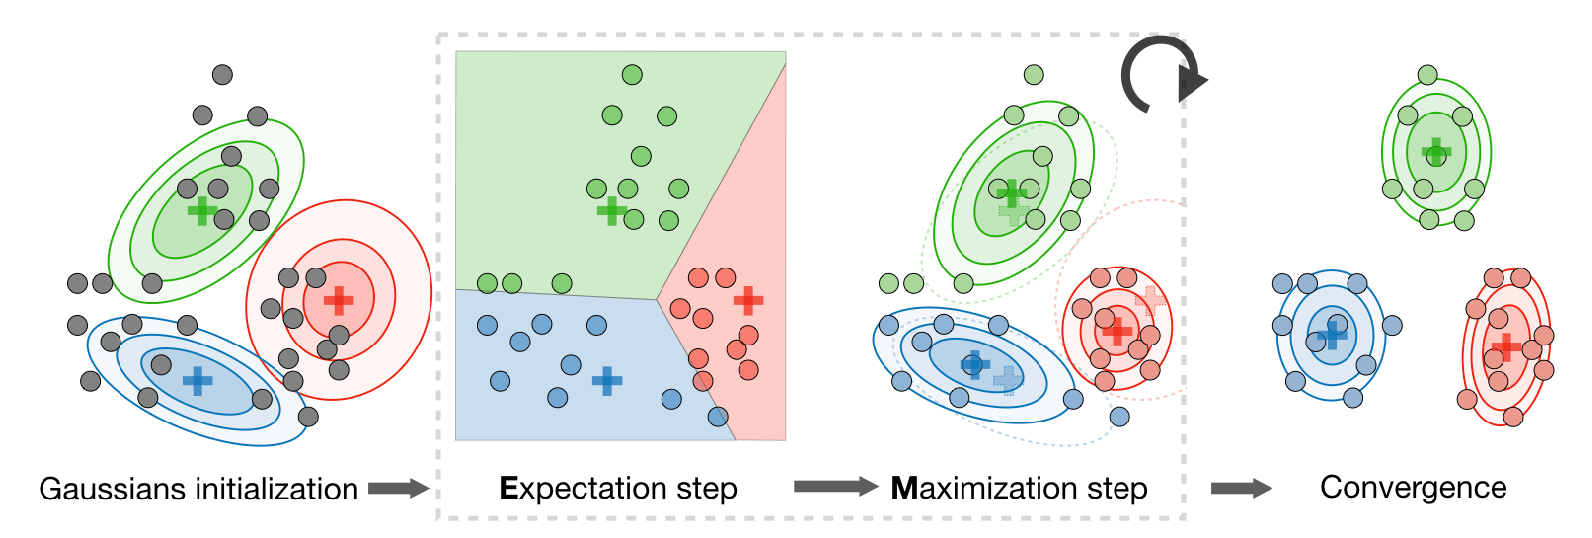
\includegraphics[width=\linewidth]{EM.png}
		Likelihood:
		\[\+L(\phi,\mu,\Sigma)=\sum_{i=1}^n\log\sum_{z^i=1}^k\Pr(x^i|z^i;\mu,\Sigma)\Pr(z^i|\phi)\]

		\section{Spectral}
		对数据有很好的表征,非凸数据;但是拓展性不好。

		Similarity: $W_{ij}=s(x_i,x_j)=\exp(-\flatfrac{\norm{x_i-x_j}^2}{2\sigma^2})$

		Graph Constructin: $\varepsilon$-neighborhood, fully connected and KNN.
		\begin{defi}
			Some useful definations:

			$d_i=\sum_{j\in V}W_{ij}$

			$\mathrm{cut}(A,B)=\sum_{i\in A,\,j\in B}W_{ij}$

			$\mathrm{cut}(A_1,A_2,\cdots,A_k)=\frac{1}{2}\sum_{i=1}^k\mathrm{cut}(A_i,\bar{A_i})$

			$\mathrm{RatioCut}(A_1,A_2,\cdots,A_k)=\frac{1}{2}\sum_{i=1}^k\mathrm{cut}(A_i,\bar{A_i})/\abs{A_i}$

			$\mathrm{Ncut}(A_1,A_2,\cdots,A_k)=\frac{1}{2}\sum_{i=1}^k\mathrm{cut}(A_i,\bar{A_i})/\mathrm{vol}(A_i)$

			Degree of the subgraph A: $\mathrm{vol}(A)=d_A=\sum_{i,j\in A} W_{ij}$

			Laplacian: $L=D-W$ where $W=\mathrm{diag_i}\qty(\sum_{(i,j)\in E}W_{ij})$
		\end{defi}
		\begin{thm}
			\[
				\mathrm{cut}(A,\bar{A})=x^TLx
				\text{ and }
				\mathrm{cut}(A_1,\cdots,A_k)=\mathrm{trace}(X^TLX)
			\]
			\texttt{Proof:}
			$\LHS=\sum_{i\in A}d_i-\sum_{i,j\in A}W_{ij}$.
		\end{thm}
		\begin{thm}Relaxation: $x\in \{0,1\}^\abs{V}\rightarrow\RR^\abs{V}$.

			$\min \mathrm{cut}(A,\bar{A}) \iff \min x^TLx=(x^TLx)/(x^Tx) \iff$ $x$为L的最小非零特征值所对应的特征向量 (\href{https://en.wikipedia.org/wiki/Rayleigh_quotient}{Rayleigh quotient Theorem})。
		\end{thm}
		\begin{defi}\textbf{Normalized} Spectral Clustering:
			\begin{itemize}
				\item
				      对拉普拉斯矩阵进行标准化操作:$L\gets D^{-0.5}LD^{-0.5}$
				\item
				      计算标准化操作后拉普拉斯矩阵最小的$k_1$个特征值对应的特征向量$F$
				\item
				      将$F$组成的矩阵按行标准化,组成$n\times k_1$的特征矩阵$P$。
				\item
				      对$P$中的每一行作为一个$k_1$维的样本,用聚类方法进行聚类。
			\end{itemize}
		\end{defi}

		\section{PCA}
		Compressing matrix $W\in\RR^{n,d}$ and recovering matrix  $U\in\RR^{d,n}$:
		$\argmin_{W,U}\sum^{n}_{i=1} \norm{x_i-UWx_i}^2$

		\begin{lemma}
			Let $(U,W)$ be a solution of Equation above. Then $U^TU=I$ and  $W=U^T$. (The columns of $U$ are orthonormal.)
		\end{lemma}

		By the fact that
		\[
			\norm{x-UU^Tx}^2=\norm{x}^2-\-{trace}(U^Txx^TU)
		\] We could rewrite the Equation as follows:
		\[
			\argmax_{U\in\RR^{d,n}:U^TU=I}\-{trace}\qty[U^T \qty(\sum^{m}_{i=1}x_ix_i^T) U]
		\]
		\begin{thm}
			Let $x_1,\cdots, x_m$ be arbitrary vectors in $\RR^d$,
			let $A = \sum^{m}_{i=1}  x_ix_i^T$,
			and let $u1,\cdots, u_n$ be $n$ eigenvectors of the matrix $A$ corresponding to the largest $n$ eigenvalues of $A$.
			Then, the solution to the PCA optimization problem given in Equation is to set $U$ to be the matrix whose columns are $u_1,\cdots,u_n$ and to set $W = U^T$.
			(More Intuition: \href{https://mathoverflow.net/questions/248198/maximizing-trace-of-mathrm-vt-mathrm-a-mathrm-v-for-mathrm-a-symmetric}{MathOverFlow})
		\end{thm}
		\begin{prf}
			Let $VDV^T$ be the spectral decomposition of  $A$ (suppose that $D_{1,1}\ge \cdots\ge D_{d,d}$) and let $B=V^TU$. We have
			\[
				\begin{aligned}
					\mathrm{trace}\qty(U^TAU)
					 & =
					\mathrm{trace}\qty(B^TDB)
					=
					\sum^{d}_{j=1} D_{j,j}\sum^{n}_{i=1} B^2_{j,i}
					\\&\le
					\max_{\*\beta\in[0,1]^d:\norm{\*\beta}\le n}\sum^{d}_{j=1} D_{j,j}\beta_j
					=
					\sum^{n}_{j=1} D_{j,j}
				\end{aligned}
			\]
			Nota Bene: $B^TB=I$ which entails  $ \sum^{d}_{j=1} \sum^{n}_{i=1} B^2_{j,i}=n $.
		\end{prf}

		\section{Dimensionality Reduction}

		\subsection{PCA}
		拟合了训练数据的长轴短轴,使得映射后得到的低维度向量分布散射最大

		\subsection{MDS}
		找到映射方向使得在低维空间中高维度样本间距离不变
		\[
			\min \sum_{i<j}\norm{\hat{x}_i-\hat{x}_j}-d_{ij}
		\]

		\subsection{ISOMAP}
		Geodesic距离 ($d_{ij}\gets$ shortest path) 能反映该数据的真正低维流形结构,保留数据集的本征几何特征。

		\subsection{Locally Linear Embedding}
		从局部的线性结构关系,恢复全局的非线性流形。假设:$\hat{x}_i=\sum_jW_{ij}x_j$ and $\sum_j W_{ij}=1$.
		\[
			\min \sum_i\norm{x_i-\sum_jW_{ij}x_j}^2
			\text{s.t.} W_{ij}=0 \text{ if }X_j\in\+N(X_i)
		\]

		\subsection{ISOMAP VS LLE}
		都保留了邻接的几何结构;都没有显式的映射函数,故使用比较麻烦;LLE需要更多的训练数据;ISOMAP计算效率高,实用性更高



		\section{Deep Learning}
		Trivial.
		\begin{md}

			\subsection{CNN}
			\[
				N=\frac{W-F+2P}{S}+1
				.\]

			\subsection{RNN}
			\[
				h_{t+1}=\-{Tanh}(W_hh_t+W_xx_{t+1})
				.\]

			\subsection{Attention}
			\[
				y=\-{SoftMax}\qty(\frac{QK^T}{\sqrt{D}})V
				.\]

			\subsection{Weight Initialization}
			\[w\gets \sqrt{\flatfrac{2}{n}}\times\-{Rand}\+N(0,1)\]

			\subsection{Activate Function}
			\[
				\-{Sigmoid}(z)=\frac{1}{1+\exp(-z)}
				\qand
				\-{Tanh}(z)=\frac{e^z-e^{-z}}{e^z+e^{-z}}
			\]

			\subsection{Batch Normalization} (BP for BN is challenging)

			Update:
			\[
				\mu = \alpha\mu + (1-\alpha)\hat{\mu}
				\qand
				\sigma^2 = \alpha\sigma^2 + (1-\alpha)\hat{\sigma}^2
				.\]

			Forward and Eval:
			\[
				x_i\gets \gamma \frac{x_i-\mu}{\sqrt{\sigma^2+\varepsilon}}+\beta
			\]

			\subsection{Momentum}
			\[
				v\gets\mu v-\alpha\dd x \qand x\gets x+v
			\]

			\subsection{Adam}
			\[
				\begin{aligned}
					m\gets\beta_1 m+(1-\beta_1)\dd x
					           & \qand
					m_t \gets \flatfrac{m}{(1-beta_1^t)}
					\\
					v\gets\beta_2 v+(1-\beta_2)\dd x^2
					           & \qand
					v_t \gets \flatfrac{v}{(1-beta_2^t)}
					\\
					x \gets x- & \frac{\alpha m_t}{\sqrt{v_t+\varepsilon}}
				\end{aligned}
			\]
		\end{md}
	\end{multicols}
\end{tiny}

\end{document}
